% Options for packages loaded elsewhere
\PassOptionsToPackage{unicode}{hyperref}
\PassOptionsToPackage{hyphens}{url}
%
\documentclass[
]{article}
\usepackage{amsmath,amssymb}
\usepackage{iftex}
\ifPDFTeX
  \usepackage[T1]{fontenc}
  \usepackage[utf8]{inputenc}
  \usepackage{textcomp} % provide euro and other symbols
\else % if luatex or xetex
  \usepackage{unicode-math} % this also loads fontspec
  \defaultfontfeatures{Scale=MatchLowercase}
  \defaultfontfeatures[\rmfamily]{Ligatures=TeX,Scale=1}
\fi
\usepackage{lmodern}
\ifPDFTeX\else
  % xetex/luatex font selection
\fi
% Use upquote if available, for straight quotes in verbatim environments
\IfFileExists{upquote.sty}{\usepackage{upquote}}{}
\IfFileExists{microtype.sty}{% use microtype if available
  \usepackage[]{microtype}
  \UseMicrotypeSet[protrusion]{basicmath} % disable protrusion for tt fonts
}{}
\makeatletter
\@ifundefined{KOMAClassName}{% if non-KOMA class
  \IfFileExists{parskip.sty}{%
    \usepackage{parskip}
  }{% else
    \setlength{\parindent}{0pt}
    \setlength{\parskip}{6pt plus 2pt minus 1pt}}
}{% if KOMA class
  \KOMAoptions{parskip=half}}
\makeatother
\usepackage{xcolor}
\usepackage[margin=1in]{geometry}
\usepackage{graphicx}
\makeatletter
\def\maxwidth{\ifdim\Gin@nat@width>\linewidth\linewidth\else\Gin@nat@width\fi}
\def\maxheight{\ifdim\Gin@nat@height>\textheight\textheight\else\Gin@nat@height\fi}
\makeatother
% Scale images if necessary, so that they will not overflow the page
% margins by default, and it is still possible to overwrite the defaults
% using explicit options in \includegraphics[width, height, ...]{}
\setkeys{Gin}{width=\maxwidth,height=\maxheight,keepaspectratio}
% Set default figure placement to htbp
\makeatletter
\def\fps@figure{htbp}
\makeatother
\setlength{\emergencystretch}{3em} % prevent overfull lines
\providecommand{\tightlist}{%
  \setlength{\itemsep}{0pt}\setlength{\parskip}{0pt}}
\setcounter{secnumdepth}{-\maxdimen} % remove section numbering
\ifLuaTeX
  \usepackage{selnolig}  % disable illegal ligatures
\fi
\IfFileExists{bookmark.sty}{\usepackage{bookmark}}{\usepackage{hyperref}}
\IfFileExists{xurl.sty}{\usepackage{xurl}}{} % add URL line breaks if available
\urlstyle{same}
\hypersetup{
  pdftitle={Econ 602 Notes},
  pdfauthor={Parker Howell},
  hidelinks,
  pdfcreator={LaTeX via pandoc}}

\title{Econ 602 Notes}
\author{Parker Howell}
\date{Last Updated: 2024-03-11}

\begin{document}
\maketitle

\hypertarget{simultaneous-move-games-of-complete-information}{%
\section{Simultaneous-move Games of Complete
Information}\label{simultaneous-move-games-of-complete-information}}

Can model these as strategic-form games

\hypertarget{def-strategic-form-game}{%
\subsubsection{Def ``strategic-form
game''}\label{def-strategic-form-game}}

A strategic-form game is a \(G = (S_i, u_i = 1, ..., I)\) such that

\begin{enumerate}
\def\labelenumi{\arabic{enumi}.}
\tightlist
\item
  \(\{1, ..., I\}\) is a set of players
\item
  \(S_i\) is a set of strategies for player \(i\)
\item
  \(u_i: \Pi_{j=1}^I S_j \rightarrow \mathbb{R}\) is a payoff function
  for player \(i\). (\(u_i\) maps from strategy profiles to real
  (integrable) numbers.)
\end{enumerate}

\textbf{Example 1:} introduce NE

\hypertarget{def-nash-equilibrium-psne}{%
\subsubsection{Def ``Nash Equilibrium
(PSNE)''}\label{def-nash-equilibrium-psne}}

Call \((s_1^*, ... ,s_I^*)\) a Nash equilibrium if, for each
\(i = 1, ..., I\)
\[u_i(s_i^*, s_{-i}^*) \geq u_i(s_i, s_{-i}), \forall s_i \in S_i.\]

\begin{quote}
``deviating to some \(s_i\) is not going to make me any better off.
\end{quote}

\hypertarget{def-best-response}{%
\subsubsection{Def ``Best Response''}\label{def-best-response}}

Say \(s_i \in S_i\) is a best response for \(i\) under \(s_{-i}\) if
\[u_i(s_i, s_{-i}) \geq u_i(s_i', s_{-i})~~~~ \forall s_i' \in S_i.\]

\hypertarget{def-best-response-correspondence}{%
\subsubsection{Def ``Best Response
Correspondence''}\label{def-best-response-correspondence}}

\(BR_i: S_{-i} \rightrightarrows S_i\) such that
\[BR_i(s_{-i}) = \{s_i \in S_i: s_i \text{ is a best response for } i \text{ under } s_{-i}\}\]

\hypertarget{remark-1}{%
\paragraph{Remark 1}\label{remark-1}}

A strategy profile is a Nash Equilibrium if and only if, for each
\(i = 1, ..., I\) \[s_i^* \in BR_i(s_{-i}).\] \textbf{Example 2}
Maximize revenue to find BR correspondence. Determine PSNE from
correspondence.

\textbf{Example 3} ``Increasing payoffs can hurt''

\begin{quote}
Difference between Game Theory and Decision Theory: In DT, increasing
payoffs cannot hurt. In GT, there are scenarios under which increasing
payoffs can hurt.
\end{quote}

\textbf{Example 4} ``incentive to hide what you are playing''

\begin{quote}
Randomization is a way of hiding what's being played.
\end{quote}

\hypertarget{def-set-of-mixed-strategies-of-i}{%
\subsubsection{\texorpdfstring{Def ``set of mixed strategies of
\(i\)''}{Def ``set of mixed strategies of i''}}\label{def-set-of-mixed-strategies-of-i}}

The set of probability measures or distributions on \(S_i\) is
\(\Delta(S_i).\)

Given \(E_i \subseteq S_i\) (event), \(\sigma(E_i)\) is the probability
that \(i\) plays a strategy in \(E_i\), if \(i\) chooses the mixed
strategy \(\sigma_i\).

\hypertarget{remark-2-infinite-strategies-have-no-atoms}{%
\paragraph{\texorpdfstring{Remark 2 ``infinite strategies have no
atoms\ldots{}''}{Remark 2 ``infinite strategies have no atoms\ldots''}}\label{remark-2-infinite-strategies-have-no-atoms}}

If \(S_i\) is finite, then
\(\sigma_i(E_i) = \sum_{s_i \in E_i} \sigma_i(s_i)\). But, this property
need not hold when \(S_i\) is infinite.

\hypertarget{remark-3}{%
\paragraph{Remark 3}\label{remark-3}}

We have (above) defined a new game called the ``mixed extension'' of
\(G = (S_i, u_i: i = 1, ..., I)\). The differences are (1) strategy sets
are now \(\Delta(S_i)\), and (2) the payoff of \(i\) from
\((\sigma_1, ..., \sigma_I)\) is \(u_i(\sigma_1, ..., \sigma_I)\).

\hypertarget{remark-4}{%
\paragraph{Remark 4}\label{remark-4}}

Consider a finite game (a game in which \(S_i\) is finite for each
\(i = 1, ..., I\).). The payoff is
\[u_i(\sigma_1, ..., \sigma_I) = \Sigma_{S_I}\cdot \cdot \cdot \Sigma_{S_1}u_i(s_1, ..., s_I)\sigma_1(s_1) \cdot \cdot \cdot \sigma_I(s_I).\]

\hypertarget{def-msne}{%
\subsubsection{Def ``MSNE''}\label{def-msne}}

Call \((\sigma_1, ..., \sigma_I)\) a ``Mixed Strategy Nash Equilibrium''
(MSNE) if, and only if, for each \(i=1, ..., I\)

\[u_i(\sigma_i^*, \sigma_{-i}^*) \geq u_i(\sigma_i, \sigma_{-i}), \forall \sigma_i \in \Delta(S_i).\]

\hypertarget{lemma-1-msne-iff-weakly-better-than-all-pure-strategies}{%
\subsubsection{\texorpdfstring{Lemma 1 ``MSNE \(\iff\) weakly better
than all pure
strategies''}{Lemma 1 ``MSNE \textbackslash iff weakly better than all pure strategies''}}\label{lemma-1-msne-iff-weakly-better-than-all-pure-strategies}}

A strategy profile \((\sigma_1, ..., \sigma_I)\) is a MSNE if, and only
if, for each \(i\)

\[u_i(\sigma_i^*, \sigma_{-i}^*) \geq u_i(s_i, \sigma_{-i}^*), \forall s_i \in S_i.\]

\hypertarget{lemma-2-msne-iff-strategy-in-support-is-best}{%
\subsubsection{\texorpdfstring{Lemma 2 ``MSNE \(\iff\) strategy in
support is
best''}{Lemma 2 ``MSNE \textbackslash iff strategy in support is best''}}\label{lemma-2-msne-iff-strategy-in-support-is-best}}

Fix a finite game \(G = (S_i, u_i: i = 1, ..., I)\).

Then \((\sigma_1, ..., \sigma_I)\) is a MSNE if, and only if, for each
\(i\) and for each \(s_i \in S_i\), with \(\sigma_i^*(s_i) > 0,\)

\[u_i(s_i, \sigma_{-i}^*) \geq u_i(r_i, \sigma_{-i}^*), \forall r_i \in S_i.\]

\hypertarget{remark-5-lemma-2-doesnt-have-the-right-context-for-the-infinite-case}{%
\paragraph{Remark 5 ``Lemma 2 doesn't have the right context for the
infinite
case''}\label{remark-5-lemma-2-doesnt-have-the-right-context-for-the-infinite-case}}

\hypertarget{cor-1-indifference-condition}{%
\subsubsection{Cor 1 ``indifference
condition''}\label{cor-1-indifference-condition}}

Fix a finite game \(G = (S_i, u_i: i = 1, ..., I)\).

If \((\sigma_1, ..., \sigma_I)\) is a MSNE and with
\(\sigma_i^*(s_i), \sigma_i^*(r_i) > 0,\) then

\[u_i(s_i, \sigma_{-i}^*) = u_i(r_i, \sigma_{-i}^*).\]

\textbf{Example 5} ``Lemma 2 doesn't work in the infinite case +
intuition for how to extend''

\hypertarget{thm-from-online-notes}{%
\subsubsection{Thm ``from online notes''}\label{thm-from-online-notes}}

\begin{enumerate}
\def\labelenumi{\arabic{enumi}.}
\tightlist
\item
  If \(\sigma_i\) induces \(F_i\), then \(F_i\) is a CDF
\item
  If \(F_i\) is a CDF, then there exists a \emph{unique} \(\sigma_i\)
  that induces \(F_i\).
\end{enumerate}

\hypertarget{remark-6-unanswered-questions}{%
\paragraph{Remark 6 ``unanswered
questions''}\label{remark-6-unanswered-questions}}

We constructed an example of a symmetric MSNE. But, we have not shown it
is the only such symmetric MSNE. Can we have a symmetric MSNE with gaps
in the support? Can we have a symmetric MSNE with atoms?

\hypertarget{remark-7-pdfcdf-technical-notes}{%
\paragraph{Remark 7 ``pdf/cdf technical
notes''}\label{remark-7-pdfcdf-technical-notes}}

omitted

\hypertarget{existence-of-pure-and-mixed-strategy-nash-equilibria}{%
\subsection{Existence of Pure and Mixed Strategy Nash
Equilibria}\label{existence-of-pure-and-mixed-strategy-nash-equilibria}}

\hypertarget{notation-mixed-best-response-correspondence}{%
\paragraph{Notation: ``Mixed Best Response
Correspondence''}\label{notation-mixed-best-response-correspondence}}

We've already seen one correspondence:
\(BR_i: S_{-i} \rightrightarrows S_i\) such that
\[BR_i(s_{-i}) = \{s_i \in S_i: s_i \text{ is a best response to } s_{-i}\}.\]

Now, we have
\(\tilde{BR}_i: \Pi_{j \neq i} \Delta (S_j) \rightrightarrows \Delta(S_i)\)
such that
\[\tilde{BR}_i(\sigma_{-i}) = \{\sigma_i \in \Delta(S_i): \sigma_i \text{ is a best response under } \sigma_{-i}\}.\]

For all players:

\[\tilde{BR}: \Pi_{i=1}^I \Delta(S_i) \rightrightarrows \Pi_{i=1}^I \Delta(S_i) \text{ such that } \tilde{BR}_i(\sigma_1, ..., \sigma_I) = \Pi_{i=1}^I \tilde{BR} (\sigma_1, ..., \sigma_{i-1}, \sigma_{i+1}, ..., \sigma_I).\]

\hypertarget{result-ne-iff-fixed-point-of-br}{%
\subsubsection{\texorpdfstring{Result ``NE \(\iff\) fixed point of
BR''}{Result ``NE \textbackslash iff fixed point of BR''}}\label{result-ne-iff-fixed-point-of-br}}

\begin{itemize}
\tightlist
\item
  \((s_1^*, ..., s_I^*)\) is a PSNE
  \(\iff (s_1^*, ..., s_I^*) \in BR(s_1^*, ..., s_I^*) \iff\) fixed
  point of \(BR\).
\item
  \((\sigma_1^*, ..., \sigma_I^*)\) is a MSNE
  \(\iff (s_1^*, ..., s_I^*) \in \tilde{BR}(\sigma_1^*, ..., \sigma_I^*) \iff\)
  fixed point of \(\tilde{BR}\).
\end{itemize}

\hypertarget{thm-kakutanis-fixed-point-thm}{%
\subsubsection{Thm ``Kakutani's fixed point
thm''}\label{thm-kakutanis-fixed-point-thm}}

Let \(X\) be nonempty compact convex set. If \(F\) is nonempty,
convex-valued, and has a closed graph, then \(F\) has a fixed point.

\hypertarget{thm-1-conditions-to-guarantee-existence-of-psne}{%
\subsubsection{Thm 1 ``conditions to guarantee existence of
PSNE''}\label{thm-1-conditions-to-guarantee-existence-of-psne}}

Fix a game where, for each \(i = 1, ..., I\), if

\begin{enumerate}
\def\labelenumi{\arabic{enumi}.}
\tightlist
\item
  there exists an \(n_i\) such that \(S_i\) is a nonempty, compact,
  convex subset of \(\mathbb{R}^{n_i}\),
\item
  \(u_i: S \rightarrow \mathbb{R}\) is continuous, and
\item
  for each \(s_{-i}\), holding \(s_i\) fixed,
  \(u_i(\cdot, s_{-i}): S_i \rightarrow \mathbb{R}\) is quasiconcave.
\end{enumerate}

\begin{quote}
nonempty: from \(S_i\) being compact and continuity of utility fn (BR
has to be nonempty)
\end{quote}

\begin{quote}
closed-graph: from continuity of \(u_i\)
\end{quote}

\begin{quote}
convex-valued (\(F\)): from quasiconcavity of
\(u_i(\cdot, s_{-i}): S_i \rightarrow \mathbb{R}\)
\end{quote}

\hypertarget{thm-2-conditions-to-guarantee-existence-of-msne}{%
\subsubsection{Thm 2 ``conditions to guarantee existence of
MSNE''}\label{thm-2-conditions-to-guarantee-existence-of-msne}}

For each finite game, there exists a MSNE.

\hypertarget{thm-3-glicksbergs-thm}{%
\subsubsection{Thm 3 ``Glicksberg's thm''}\label{thm-3-glicksbergs-thm}}

Fix a game, \(G\) where, for each \(i\),

\begin{enumerate}
\def\labelenumi{\arabic{enumi}.}
\tightlist
\item
  \(S_i\) is compact metric space, and
\item
  \(u_i: S \rightarrow \mathbb{R}\) is continuous.
\end{enumerate}

Then \(G\) has a MSNE.

\hypertarget{remark-8}{%
\paragraph{Remark 8}\label{remark-8}}

Glicksberg's thm doesn't tell us that the assumptions of compactness and
continuity are interesting. E.g., first-price auctions are
discontinuous.

\hypertarget{remark-9}{%
\paragraph{Remark 9}\label{remark-9}}

Glicksberg's thm only tells us there is some equilibrium--there may be
many.

\hypertarget{remark-10}{%
\paragraph{Remark 10}\label{remark-10}}

Existence results are most useful if there are qualitative results of
how equlibria vary with interesting parameters of the model/game.

\hypertarget{rationalizability-and-iterated-dominance}{%
\section{Rationalizability and Iterated
Dominance}\label{rationalizability-and-iterated-dominance}}

\textbf{Example 1} ``motivation for beliefs: can have wrong beliefs
now.''

\hypertarget{term-belief}{%
\paragraph{Term ``belief''}\label{term-belief}}

Belief of player \(i\): \(\mu_i \in \Delta(S_{-i})\)

\hypertarget{def-best-response-with-beliefs}{%
\subsubsection{Def ``best response with
beliefs''}\label{def-best-response-with-beliefs}}

Fix a nonempty set \(Q_i \subseteq S_i\). Say \emph{\(s_i\) is a best
response under \(\mu_i\) given \(Q_i\)} if \(s_i \in Q_i\) and
\[\int_{S_{-i}} u_i(s_i, s_{-i})d\mu_i \geq \int_{S_{-i}} u_i(r_i, s_{-i})d\mu_i, ~\forall r_i \in Q_i.\]
Say \emph{\(s_i\) is a best response under \(\mu_i\)} if it is a best
response under \(\mu_i\) given \(S_i\).

Or, in discrete settings:
\[\sum_{s_{-i} \in S_{-i}} u_i(s_i, s_{-i})\mu_i(s_{-i}) \geq \sum_{s_{-i} \in S_{-i}} u_i(r_i, s_{-i})\mu_i(s_{-i}), ~\forall r_i \in Q_i.\]

\hypertarget{def-justifiable}{%
\subsubsection{Def ``justifiable''}\label{def-justifiable}}

Fix a nonempty (candidate subset) \(Q_{-i} \subseteq S_{-i}\). Say
\emph{\(s_i\) is justifiable given \(Q_{-i}\)} if there exists
\(\mu_i \in \Delta(S_{-i})\) such that

\begin{enumerate}
\def\labelenumi{\arabic{enumi}.}
\tightlist
\item
  \(s_i\) is a best response under \(\mu_i\) and
\item
  \(\mu_i(Q_{-i})=1\).
\end{enumerate}

Say \(s_i\) is \emph{justifiable} if it is justifiable given \(S_{-i}\).

\hypertarget{def-rationalizable-sets}{%
\subsubsection{Def ``rationalizable
sets''}\label{def-rationalizable-sets}}

Let \(R_i^0 = S_i; R_{-i}^0 = S_{-i}.\)

Inductively define sets \(R_i^m\) and \(R_{-i}^m\) such that

\begin{itemize}
\tightlist
\item
  \(R_i^{m+1} = \{s_i \in S_i: s_i \text{ is justifiable given } R_{-i}^m\}\),
  and
\item
  \(R_{-i}^{m+1} = \Pi_{j \neq i}R_{j}^{m+1}\).
\end{itemize}

Additional notation:

\begin{itemize}
\tightlist
\item
  \(R_i^\infty = \cap_{m\geq 0}\) is the set of rationalizable
  strategies for \(i\).
\item
  \(R^\infty = \Pi_{i=1}^I R_i^\infty\) is the set of rationalizable
  strategy profiles.
\item
  \(R^m = \Pi_{i=1}^I R_i^m\) is the set of \(m-\)rationalizable
  strategy profiles.
\end{itemize}

\textbf{Examples 2-4} ``which strategies are justifiable?''

\hypertarget{def-undominated}{%
\subsubsection{Def ``(un)dominated''}\label{def-undominated}}

Fix \(Q_1, ..., Q_I\) where each \(Q_j \subseteq S_j\).

Say \emph{\(s_i\) is dominated given \(\Pi_{j=1}^I Q_j\)} if
\(s_i \in Q_i\) and there exists a \(\sigma_i \in \Delta(S_i)\) such
that
\[u_i(\sigma_i,s_{-i}) > u_i(s_i,s_{-i}),~\forall s_{-i} \in \Pi_{j \neq i}^I Q_j.\]

Say \emph{\(s_i\) is undominated given \(\Pi_{j=1}^I Q_j\)} if it is not
dominated given \(\Pi_{j=1}^I Q_j\).

Say \emph{\(s_i\) is (un)dominated} if it is (un)dominated given \(S\).

\hypertarget{def-undominated-sets}{%
\subsubsection{Def ``undominated sets''}\label{def-undominated-sets}}

Let \(U_i^0 = S_i.\)

Inductively define \(U_i^m\) such that
\[U_i^{m+1} = \{s_i \in S_i: s_i \text{ is undominated given } U_{-i}^m\}.\]

Additional notation:

\begin{itemize}
\tightlist
\item
  \(U_i^\infty = \cap_{m\geq 0}U_i^m\) is the set of undominated
  strategies for \(i\).
\item
  \(U^m = \Pi_{i=1}^I R_i^m\) is the set of \(m-\)undominated strategy
  profiles.
\item
  \(U^\infty = \Pi_{i=1}^I U_i^\infty\) is the set of \emph{iteratively
  undominated} (IU) strategy profiles.
\end{itemize}

\hypertarget{thm-1-rm-um}{%
\subsubsection{\texorpdfstring{Thm 1
``\(R^m = U^m\)''}{Thm 1 ``R\^{}m = U\^{}m''}}\label{thm-1-rm-um}}

Fix a finite game. \(R^m = U^m, ~\forall m.\)

\hypertarget{prop-1-justifiable-iff-undominated}{%
\subsubsection{\texorpdfstring{Prop 1 ``justifiable \(\iff\)
undominated''}{Prop 1 ``justifiable \textbackslash iff undominated''}}\label{prop-1-justifiable-iff-undominated}}

Fix a finite game. A strategy \(s_i\) is justifiable if, and only if, it
is undominated.

\hypertarget{def-hyperplane}{%
\subsubsection{Def ``Hyperplane''}\label{def-hyperplane}}

A hyperplane in \(\mathbb{R}^n\) is a set of the form
\[H[\vec{p}, \alpha] = \{\vec{x} \in \mathbb{R}^n: \vec{p} \cdot \vec{x}= \alpha\}\]
for \(\vec{p} \in \mathbb{R}^n \setminus \{0\}\) and
\(\alpha \in \mathbb{R}\).

\hypertarget{def-supporting-hyperplane}{%
\subsubsection{Def ``supporting
hyperplane''}\label{def-supporting-hyperplane}}

Fix \(A \subseteq \mathbb{R}^n\) and \(\vec{x} \in A\). Say
\(\vec{p} \in \mathbb{R}^n\) (with \(\vec{p}\neq \vec{0}\))
\emph{supports \(A\) at \(\vec{x}\)} if
\[\vec{p} \cdot \vec{x} \geq \vec{p} \cdot \vec{y}, \forall y \in A.\]

Say \(H[\vec{p}, \alpha]\) supports \(A\) at \(\vec{x}\) if \(\vec{p}\)
supports \(A\) at \(\vec{x}\) and \(\vec{p} \cdot \vec{x} = \alpha\).

\hypertarget{thm-supporting-hyperplane-theorem}{%
\subsubsection{Thm ``Supporting Hyperplane
Theorem''}\label{thm-supporting-hyperplane-theorem}}

Let \(A \subseteq \mathbb{R}^n\), convex and \(\vec{x} \in A\). There
exists some \(\vec{p} \in \mathbb{R}^n\) (with \(\vec{p}\neq \vec{0}\))
such that \(\vec{p}\) supports \(A\) at \(\vec{x}\) if and only if
\(\vec{x} \notin int(A)\). (i.e., \(\vec{x} \in\) boundary(\(A\)))

\textbf{Example 6} ``weakly dominated''

\hypertarget{lemma-1-later-sets-subsets-of-earlier-subsets}{%
\subsubsection{Lemma 1 ``later sets subsets of earlier
subsets''}\label{lemma-1-later-sets-subsets-of-earlier-subsets}}

For each \(i = 1, ..., I\) and each \(m\geq 0\),
\(R_i^{m+1} \subseteq R_i^m\).

\hypertarget{cor-0.1-rationalizable-set-stops-shrinking-at-some-point}{%
\subsubsection{Cor 0.1 ``rationalizable set stops shrinking at some
point''}\label{cor-0.1-rationalizable-set-stops-shrinking-at-some-point}}

If the game is finite, there exists some number \(M\) such that
\(R^m = R^M\) for all \(m \geq M\).

\textbf{Example 0.1} NEED TO WORK THROUGH

\hypertarget{prop-1-nonempty-rationalizable-set-exists-if-compact-and-continuous}{%
\subsubsection{Prop 1 ``nonempty rationalizable set exists if compact
and
continuous''}\label{prop-1-nonempty-rationalizable-set-exists-if-compact-and-continuous}}

Fix a game \(G = (S_i, u_i: i = 1, ..., I)\) where each \(S_i\) is a
compact metrics space and each \(u_i\) is continuous. Then the set of
rationalizable strategy profiles is nonempty.

\hypertarget{def-weakly-dominated}{%
\subsubsection{Def ``Weakly Dominated''}\label{def-weakly-dominated}}

Fix non-empty sets \(Q_1, ..., Q_I\). Say \(s_i\) is \emph{weakly
dominated given} \(\Pi_{j=1}^I Q_j\) if \(s_i \in Q_i\) and there exists
\(\sigma_i \in \Delta(Q_i)\) so that

\begin{enumerate}
\def\labelenumi{\arabic{enumi}.}
\tightlist
\item
  \(u_i(\sigma_i, s_{-i}) \geq u_i(s_i, s_{-i})\) for each
  \(s_{-i} \in \Pi_{j\neq i} Q_j\), and
\item
  \(u_i(\sigma_i, s_{-i}) > u_i(s_i, s_{-i})\) for some
  \(s_{-i} \in \Pi_{j\neq i} Q_j\).
\end{enumerate}

Say \(s_i\) is \emph{weakly dominated} if it is weakly dominated given
\(S\).

\hypertarget{def-iterated-weak-dominance}{%
\subsubsection{Def ``Iterated Weak
Dominance''}\label{def-iterated-weak-dominance}}

Set \(W_i^0 = S_i\). Inductively define \(W_i^m\) such that
\[W_i^{m+1} = \{s_i \in W_i^m: s_i \text{ is not weakly dominated given } \Pi^{I}_{j=1}W_j^m\}.\]

Then \(W_i^{m+1}\) is the set of strategies of \(i\) that survive
\((m+1)\) rounds of iterated weak dominance.

Set \(W_i^\infty = \cap_{m\geq 0}W_i^m\). Then
\(W^\infty = \Pi_{i=1}^I W_i^\infty\) is the set of strategy profiles
that survive iterated weak dominance.

\hypertarget{sequential-games-of-complete-information}{%
\section{Sequential Games of Complete
Information}\label{sequential-games-of-complete-information}}

\textbf{Example 1} Entrant (E) can \emph{enter} or stay \emph{out}. If E
enters, then incumbent monopolist (I) can \textbf{F}ight or
\textbf{A}cquiesce.

Profits to (E, I), subject to \(M \geq 2\), are:

\begin{itemize}
\tightlist
\item
  (out, \(*\)): \((0,M)\)
\item
  (enter, A): \((\frac{M}{2},\frac{M}{2})\)
\item
  (enter, F): \((-1,1)\)
\end{itemize}

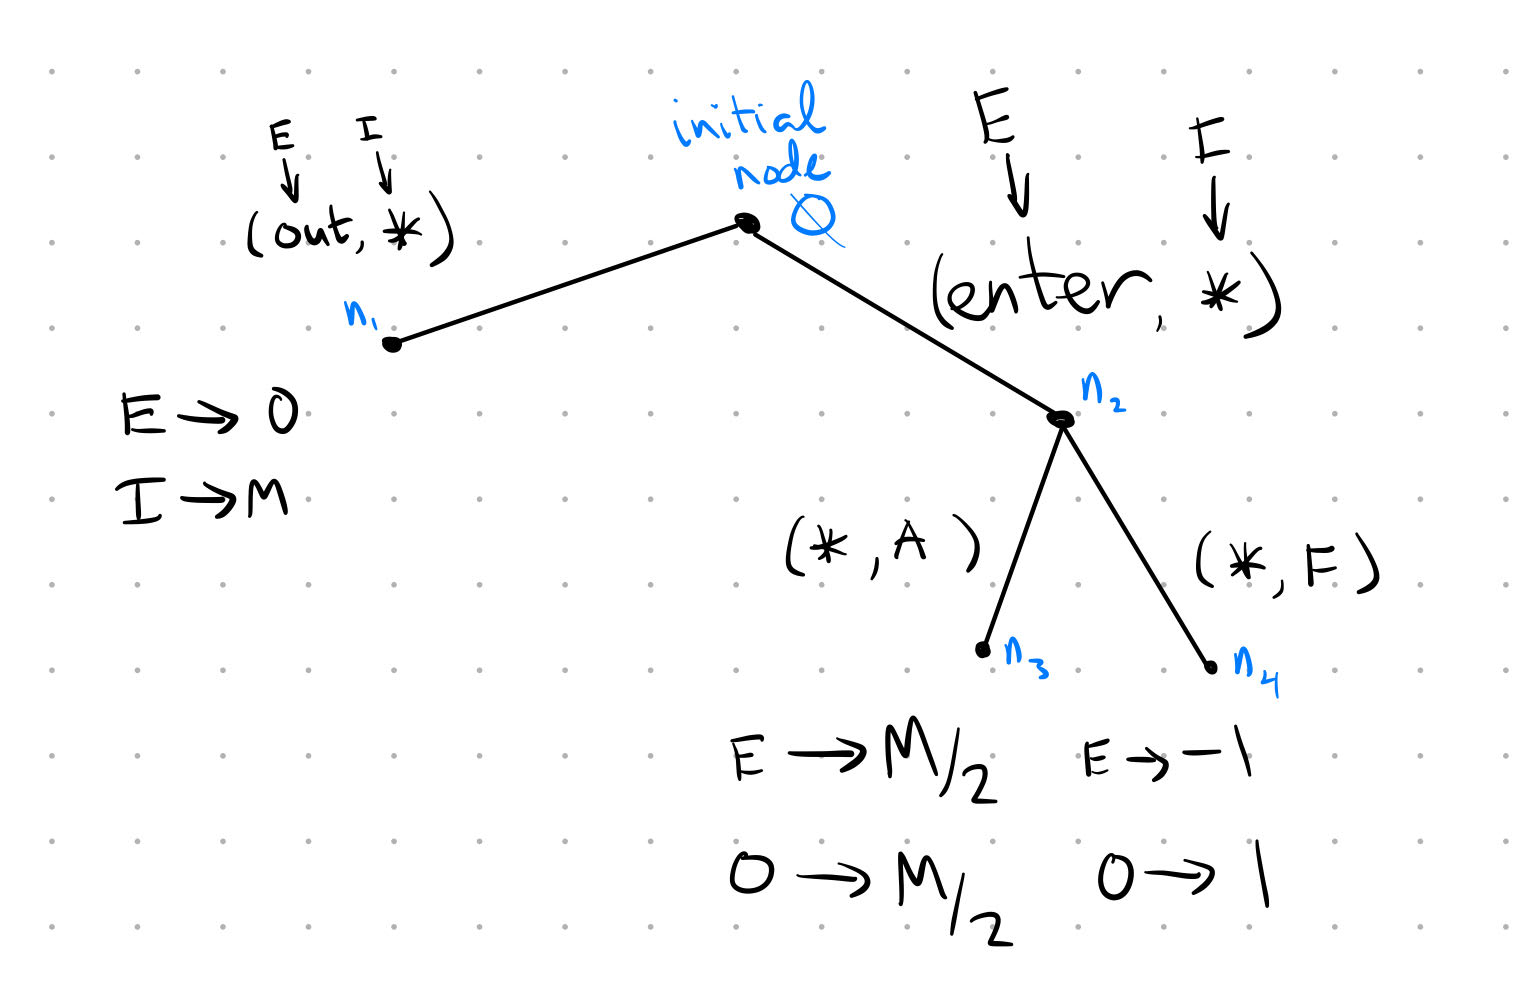
\includegraphics{src/visualization.jpg}

\hypertarget{remark-1-1}{%
\paragraph{Remark 1}\label{remark-1-1}}

Some people will see an example like example 1 and conclude ``the
strategic form game does not suffice.'' This is incorrect. We will see
(later) that the problem is the solution concept of Nash Equilibrium,
not the strategic form, per se.

Visualization vs Formalization - omitted for now.

\hypertarget{def-extensive-form-model-a-sequential-game-as-an-extensive-form-game}{%
\subsubsection{Def Extensive Form (model a sequential game as an
extensive-form
game)}\label{def-extensive-form-model-a-sequential-game-as-an-extensive-form-game}}

We model a sequential game as an extensive form game:
\(\Gamma = (A1, ..., A_J; N; H_1, ..., H_I; U_1, ..., U_I)\).

\textbf{Extensive-Form 1:} Players \(1, ..., I\)

\textbf{Extensive-Form 2:} Action Sets \((A_1, ..., A_I)\), where
\(A_i\) is the set of actions player i can choose \emph{somewhere} in
the game. E.g., \(A_E = \{O, E, *\}, A_I = \{F, A, *\}\)

\textbf{Extensive-Form 3:} Nodes \(N=\) set of nodes.

\begin{quote}
Each non-terminal node, \(n\) is associated with a set \(A_i(n)=\)set of
actions of \(i\) that can be played at \(n\).
\end{quote}

\begin{quote}
\(\Pi_{i=1}^I A_i(n)=\)set of action profiles that can be played at
\(n\).
\end{quote}

\begin{quote}
\(A_i(n) \neq \phi\) but might be a singleton (e.g.,
\(A_i(\phi) = \{*\}\)).
\end{quote}

\begin{quote}
\$Z = \$ set of terminal nodes. We don't define \(A_i(n)\) at terminal
nodes.
\end{quote}

Think of nodes as being defined by sequences of action profiles. E.g.,

\begin{itemize}
\tightlist
\item
  initial node = the empty sequence, \(\phi\), because nothing has been
  played.
\item
  \(n_1 = (O, *)\)
\item
  \(n_2 = (E, *)\)
\item
  \(n_3 = ((E, *), (*, A))\)
\item
  \(n_4 = ((E, *), (*, F))\)
\end{itemize}

\textbf{Extensive-Form 4:} Information Sets \(H_1, ..., H_I\)

\begin{itemize}
\tightlist
\item
  \(H_i\) is the set of information sets for \(i\)

  \begin{itemize}
  \tightlist
  \item
    if \(h_i \in H_i\) then \(h_i \subseteq N \setminus Z\)
  \end{itemize}
\item
  \(H_i\) forms a partition of \(N \setminus Z\)
\item
  If \(n, n' \in h_i, h_i \in H_i\) then \(A_i(n) = A_i(n')\)
\end{itemize}

\textbf{Extensive-Form 5:} Payoff Functions

Mapped from terminal nodes to numbers: \[U_i: Z \rightarrow \mathbb{R}\]

Typically add

\begin{enumerate}
\def\labelenumi{\arabic{enumi}.}
\tightlist
\item
  No absentmindedness (rules out forgetting if you moved at all), and
\item
  Perfect recall (rules out a situation where I remember I moved, but
  not what I chose).
\end{enumerate}

\hypertarget{term-no-absentmindedness}{%
\paragraph{Term ``No
absentmindedness''}\label{term-no-absentmindedness}}

Intuitively, this requires that \(i\) does not forget that she made
\emph{some} previous choice. So, there is no \(h_i \in H_i\) with
\(n, n' \in h_i\) so that \(n\) strictly precedes \(n'\). (If there were
such an \(n\) and \(n'\), then at \(n'\) player \(i\) has forgotten that
she was at \(n\) and made a choice.)

\hypertarget{term-perfect-recall}{%
\paragraph{Term ``Perfect recall''}\label{term-perfect-recall}}

Intuitively, this requires that \(i\) remembers \emph{which} previous
choice they made. So there is no situation where, say, \(i\) knows they
moved previously but cannot remember if they chose \(l\) or \(r\).

\hypertarget{def-specific-games-of-interest}{%
\subsubsection{Def ``Specific Games of
Interest''}\label{def-specific-games-of-interest}}

\begin{enumerate}
\def\labelenumi{\arabic{enumi}.}
\tightlist
\item
  Simultaneous-move games: the only non-terminal node is \(\phi\).
\item
  Games with observable actions: for each player, \(i\), each
  \(h_i \in H_i\) is a singleton.
\item
  Perfect-info games: games with observable actions where, at each info
  set there is at most one active player
\end{enumerate}

\hypertarget{term-active-player}{%
\paragraph{Term ``Active player''}\label{term-active-player}}

\[|A_i(n)| \geq 2\]

\textbf{Example 2} ``Introduces (derived) strategies''

\hypertarget{def-strategy}{%
\subsubsection{Def ``strategy''}\label{def-strategy}}

A strategy for \(i\) is an \(s_i: H_i \rightarrow A_i\) such that
\(s_i(h_i) \in A_i(h_i)\).

(Note: we've only allowed pure strategies so far, but mixed will fit in
later).

\begin{quote}
A strategy is a full contingency plan of action. It tells me what to do
at each info set.
\end{quote}

\begin{quote}
A strategy will specify 1 action at EACH \(h_i \in H_i\) where \(i\) is
making a choice.
\end{quote}

\hypertarget{term-path-function}{%
\paragraph{Term ``Path function''}\label{term-path-function}}

\[\zeta: S \rightarrow Z\]

\hypertarget{term-strategic-form-payoff-function}{%
\paragraph{Term ``strategic-form payoff
function''}\label{term-strategic-form-payoff-function}}

\[u_i: S \rightarrow \mathbb{R} \text{ such that } u_i(s) = U_i(\zeta(s)),  \forall s\in S.\]
\textbf{Example 3:} In a simultaneous game: \(S_i = A_i\).

\textbf{Analyzing games: Solution concepts}

\begin{itemize}
\tightlist
\item
  we can always write down the strategic form of the game and solve by
  NE. The problem is that NE doesn't require sequentially optimal
  behavior.
\item
  instead, we need sequential optimality and for the players to believe
  other players are also sequentially optimizing.
\end{itemize}

\hypertarget{def-subgame}{%
\subsubsection{Def ``subgame''}\label{def-subgame}}

We identify subgames with singleton information sets, \(h = \{n\}\)
where

\begin{enumerate}
\def\labelenumi{\arabic{enumi}.}
\tightlist
\item
  \(h\) is an information set for all \(i\), and
\item
  if \(n'\) follows \(n\), and \(n' \in h_i'\), then all nodes in
  \(h_i'\) follow \(n\).
\end{enumerate}

\textbf{Facts about subgames:}

\begin{itemize}
\tightlist
\item
  Each subgame is associated with a new strategic-form game which is
  associated with \(h\). We call this new, strategic form game \(G^h\)
  (Remember, \(G\) for strategic/normal, and \(\Gamma\) for
  sequential/extensive).
\item
  Intuitively, \(G^h\) consists of strategies in the \emph{original}
  strategic-form game that allow \(h\).
\item
  Given \(s_i \in S_i\), write \(s_i^h\) for a (potentially different)
  strategy that allows \(h\) and otherwise agrees with \(s_i\).
\end{itemize}

\hypertarget{def-subgame-perfect-equilibrium-spe}{%
\subsubsection{Def ``Subgame Perfect Equilibrium
(SPE)''}\label{def-subgame-perfect-equilibrium-spe}}

Call \((s_1^*, ..., s_I^*)\) a \emph{subgame perfect equilibrium} (SPE)
if, for each subgame \(h\), \((s_1^{*h}, ..., s_I^{*h})\) is a (pure
strategy) Nash equilibrium of \(G^h\).

\textbf{Example 3} Battle of the sexes with an outside option.

\hypertarget{object-backward-induction-algorithm}{%
\subsubsection{Object ``Backward-induction
algorithm''}\label{object-backward-induction-algorithm}}

\begin{enumerate}
\def\labelenumi{\arabic{enumi}.}
\tightlist
\item
  Look at each last nonterminal node and the player who moves there.
  Find \emph{an} action that is a best response for that player at that
  node.
\item
  Look at nonterminal nodes that are followed only by ``last nonterminal
  nodes''. Find an action (for the player who moves at such a node) that
  is a best response given the behavior specified in step 1.
\item
  Repeat until we reach the start of the game.
\end{enumerate}

This delivers an action associated with each information set. Collect
these actions into strategies of each player and we have an SPE.

(re-run the algorithm for each action that is a best response at each
node to find the full set of SPE)

\begin{quote}
Caution: Backward-induction applies only to perfect information games.
\end{quote}

\textbf{Example 4} ``SPE without observable actions may look peculiar''

\begin{quote}
Important point: for the purpose of iterated weak dominance, it suffices
to look at the ``reduced strategic form''
\end{quote}

\hypertarget{term-reduced-strategic-form}{%
\paragraph{Term ``reduced strategic
form''}\label{term-reduced-strategic-form}}

The strategic form that collapses all realization-equivalent strategies
into one ``strategy''

\hypertarget{def-behavioral-strategy}{%
\subsubsection{Def ``behavioral
strategy''}\label{def-behavioral-strategy}}

A \emph{behavioral strategy} of \(i\) is a
\(b_i: H_i \rightarrow \Delta(A_i)\) such that
\[\forall h_i \in H_i, b_i(h_i)(A_i(h_i))=1.\]

E.g., \(b_2(h)(l) = P(l|h) = \frac{1}{4} + \frac{1}{2}\) and
\(b_2(h')(l) = P(l|h') = \frac{1}{4} + \frac{1}{8}\).

\textbf{Example 5} Extending SPE to behavioral strategies (note: we do
this in example only because the notation is cumbersome.)

\hypertarget{misc}{%
\section{Misc}\label{misc}}

\hypertarget{def-pareto-dominate}{%
\subsubsection{Def ``pareto dominate''}\label{def-pareto-dominate}}

Say a strategy profile \((s_1', ..., s_I')\) Pareto dominates
\((s_1, ..., s_I)\) if

\begin{enumerate}
\def\labelenumi{\arabic{enumi}.}
\tightlist
\item
  for all \(i\), \(u_i(s_1', ..., s_I') \geq u_i(s_1, ..., s_I)\) and
\item
  for some \(i\), \(u_i(s_1', ..., s_I') > u_i(s_1, ..., s_I)\).
\end{enumerate}

\end{document}
